\documentclass{beamer}
\usepackage{textcomp}
\usepackage[utf8]{inputenc} 
\usepackage[T1]{fontenc}
\usepackage{lmodern}

%\usepackage{multimedia}
\usepackage{graphicx}
\usepackage[french]{babel}
\usetheme{PaloAlto}
\usefonttheme{serif}
\usefonttheme{structurebold}

\title[Tangram]{Projet de résolution du casse tête du Tangram}
%\logo{\includegraphics[width=1.5cm]{logo_utbm.png}}
\author[]{Adrien BERTHET - Paul LOCATELLI - Pierre ROGNON}
\institute[UTBM]{Université de Technologies de Belfort-Montbéliard}
\date{18 juin 2013}
%\addtobeamertemplate{footline}{~\hspace*{12cm}\insertframenumber/\inserttoœtalframenumber}


\usepackage[absolute,showboxes,overlay]{textpos}     % déclaration du package
\textblockorigin{0px}{0px}                               % origine des positions
\TPshowboxesfalse  
 % n'affiche pas le contour des textblock

\AtBeginSection[]
{
  \begin{frame}<beamer>
    \frametitle{Sommaire}
{\scriptsize\tableofcontents[currentsection]
}
  \end{frame}
}


\begin{document}

\begin{frame}{}
	
	\maketitle	
	
\end{frame}

	\section*{Introduction}

\begin{frame}{Introduction}

	Pourquoi le Tangram ?
	\begin{columns}[c]
	
	\begin{column}{5cm}
   		\begin{itemize}
			\item intérêt du jeu;
			\item symbole pour l'intelligence artificielle;
			\item diversité des configurations existantes.
		\end{itemize}
  	\end{column}
	\begin{column}{5cm}
		\includegraphics[width=5cm]{tangram}
  	\end{column}
	
	\end{columns}
    	
\end{frame}


	\section{Analyse du casse-t\^ete}
	
		\subsection{Placement d'une pièce dans un modèle}

\begin{frame}{Placement d'une pièce}

	\begin{columns}[c]
		\begin{column}{4cm}
    		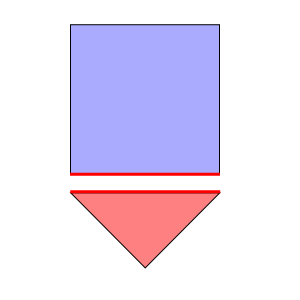
\includegraphics[width=5cm]{place_figure_exacte_match}
  		\end{column}
		\begin{column}{6.5cm}
			\begin{itemize}
				\item trouver les positions adéquates pour une pièce dans un modèle;
				\item éviter de tester toutes les solutions pour une meilleure efficacité;
				\item test des arêtes correspondant à un côté du modèle;
				\item permet de couvrir de nombreux cas.
			\end{itemize}
  		\end{column}
  		
	\end{columns}

\end{frame}

\begin{frame}{Placement d'une pièce}

	\begin{columns}[c]
		\begin{column}{4cm}
    		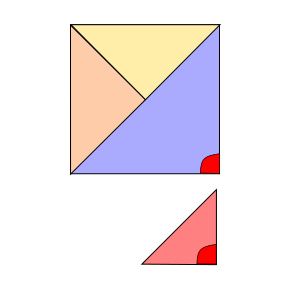
\includegraphics[width=5cm]{place_figure_probleme_angle_match}
  		\end{column}
		\begin{column}{6.8cm}
			\begin{itemize}
				\item couvre une autre partie des cas non adaptée à la première méthode;
				\item cherche des correspondances d'angles;
				\item ne permet pas de savoir si la pièce entre dans le modèle.
			\end{itemize}
  		\end{column}
  		
	\end{columns}

\end{frame}

\begin{frame}{Placement d'une pièce}

	\begin{columns}[c]
		\begin{column}{4cm}
    		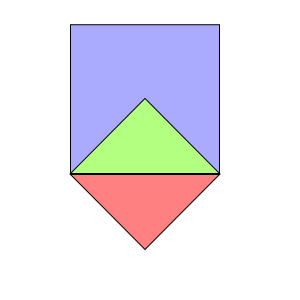
\includegraphics[width=5cm]{place_figure_probleme_symetrie_1}
  		\end{column}
		\begin{column}{6.5cm}
			\begin{itemize}
				\item la base ne permet pas d'indiquer le sens de la figure;
				\item translation éventuellement nécessaire;
				\item vérification de l'appartenance de tous les points de la pièce au modèle.
			\end{itemize}
  		\end{column}
  		
	\end{columns}

\end{frame}

\begin{frame}{Placement d'une pièce}

	\begin{itemize}
		\item une position identifiée comme correcte, une comme incorrecte;
		\item algorithme générant l'ensemble des solutions possibles;
		\item passe son résultat au prédicat suivant.
	\end{itemize}

\end{frame}

	\subsection{Soustraction d'une pièce}

\begin{frame}{Soustraction d'une pièce}

	\begin{itemize}
		\item deuxième étape, permettant la récursivité;
		\item renvoie un nouveau modèle sans la pièce placée;
		\item utilisation des arêtes nécessaires;
		\item recherche d'une arête commune.
	\end{itemize}

	\begin{center}
		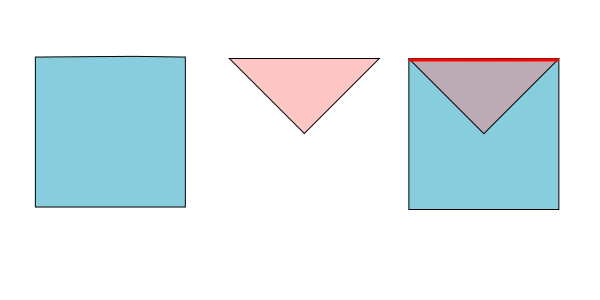
\includegraphics[width=7cm]{soustraction_arete_1}
	\end{center}

\end{frame}

\begin{frame}{Soustraction d'une pièce}

	\begin{itemize}
		\item insertion des arêtes de la pièce entre celles du modèle;
		\item vérification du sens de la pièce pour un éventuel retournement;
		\item élimination d'arêtes présentes en double;
		\item "nettoyage" des points. 
	\end{itemize}
	
	\begin{center}
		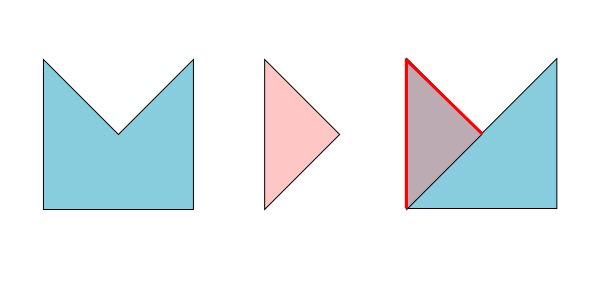
\includegraphics[width=7cm]{soustraction_arete_2}
	\end{center}

\end{frame}

\begin{frame}{Soustraction d'une pièce}

	\begin{itemize}
		\item le problème des points résolu par l'utilisation d'arêtes;
		\item suppression automatique de points et arêtes parasites;
		\item cas d'arrêt par renvoi d'un modèle vide.
	\end{itemize}

\end{frame}

	\subsection{Algorithme profondeur d'abord}
	
\begin{frame}{Profondeur d'abord: analyse de la recherche}

	\begin{itemize}
		\item problème modélisable par un arbre de recherche;
		\item arbre complexe du fait du nombre de placements possibles;
		\item étapes de résolution:
		\begin{enumerate}
			\item sélection d'une pièce;
			\item choix d'une position possible;
			\item sélection de la pièce suivante;
			\item arrêt au niveau de profondeur 7.
		\end{enumerate}
	\end{itemize}

\end{frame}

\begin{frame}{Profondeur d'abord: choix de la recherche}

	\begin{itemize}
		\item plusieurs solutions possible dans la quasi totalité des cas;
		\item but = converger vers une solution rapidement;
		\item profondeur d'abord: choix idéal;
		\item étend le nœud du graphe et ses successeurs jusqu'au nœud but.
	\end{itemize}

\end{frame}

	\section{Représentation informatique du problème}
	
		\subsection{Structure de données}
	
\begin{frame}{Structure de données}

	\begin{itemize}
		\item représentation des figures dans un repère orthonormé;
		\item coordonnées réunies en points;
		\item figure représentée par une liste de points;
		\item ordre des points importants;
		\item modèle structuré par une liste de figures.
	\end{itemize}

\end{frame}

		\subsection{Espace d'états}
		
\begin{frame}{Espace d'états}

	\begin{columns}[c]
		\begin{column}{4cm}
    		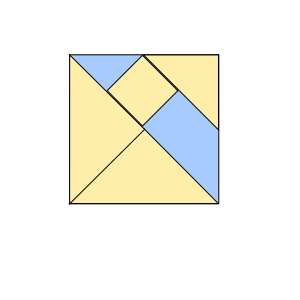
\includegraphics[width=5cm]{representation_sousfigure}
  		\end{column}
		\begin{column}{6.5cm}
			Chaque état contient:
			\begin{itemize}
				\item les pièces à placer;
				\item les coordonnées du modèle à remplir;
				\item les pièces placées.
			\end{itemize}
  		\end{column}
	\end{columns}

\end{frame}

\begin{frame}{Espace d'états}

	\begin{itemize}
		\item $Pieces$ défini dans l'ensemble des pièces disponibles;
		 \item $PiecesPlacees$ défini de la même manière;
		 \item $Modele$ défini par des points compris dans l'espace des coordonnées de base.
	\end{itemize}

\end{frame}

		
		\subsection{Système de production}
		
\begin{frame}{Système de production}

	\begin{itemize}
		\item contraintes sur les pièces placées;
		\item règles différant de la configuration du Tangram;
		\item néanmoins, règles communes concernant les coordonnées:\\
		chaque point d'une pièce dans $PiecesPlacees$ doit être dans la surface de $Modele$ à un état antérieur.
	\end{itemize}

\end{frame}

	\section{Résultat obtenus}
	
		\subsection{Avancement de la résolution}
	
\begin{frame}{Avancement de la résolution}

	\begin{itemize}
		\item résolution totale non obtenue;
		\item dû à des problèmes sur les parties géométriques du Tangram;
		\item fonctionnement effectif sur des cas simples
	\end{itemize}
	
\end{frame}

		\subsection{Exemples}

\begin{frame}{Des exemples}

	Les deux premières pièces du Tangram "carré":\\ \ \\ \ \\
	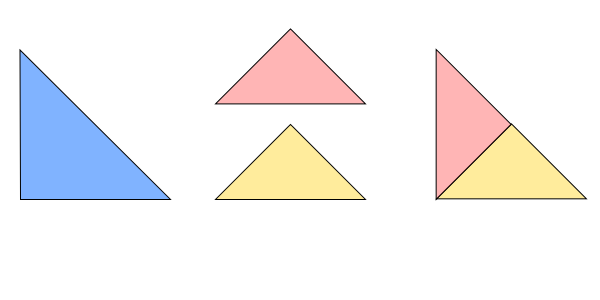
\includegraphics[width=10cm]{resultat_1}

\end{frame}

\begin{frame}{Des exemples}

	Un cas dérivé avec trois triangles:\\ \ \\ \ \\
	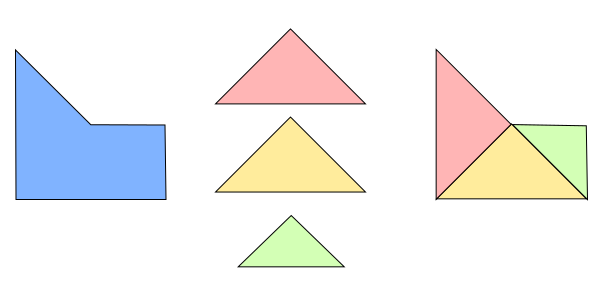
\includegraphics[width=10cm]{resultat_2}

\end{frame}

	\section{Problèmes rencontrés}
	
\begin{frame}{Problèmes rencontrés}

	\begin{itemize}
		\item peu de données sur le problème;
		\item problèmes d'ordre géométriques difficiles à modéliser;
		\item de nombreux cas particuliers;
		\item un choix de modélisation initial discutable finalement.
	\end{itemize}

\end{frame}


	\section{Conclusion}
	
\begin{frame}{Conclusion}

	\begin{itemize}
		\item projet intéressant sur le plan du sujet;
		\item des difficultés mais un résultat satisfaisant;
		\item mise en pratique du Prolog intéressante.
	\end{itemize}

\end{frame}
	

\end{document}


